\documentclass[11pt,a4paper]{article}
\usepackage[czech]{babel}
\usepackage[utf8]{inputenc}
\usepackage[T1]{fontenc}
\usepackage[top=3cm, left=2cm, text={17cm, 24cm}]{geometry}
\usepackage{graphicx}
\usepackage{caption}
\usepackage{subcaption}
\usepackage{amsmath}
\usepackage{multirow}
\usepackage[bookmarksopen,colorlinks,plainpages=false,urlcolor=blue,unicode]{hyperref}
\usepackage{url}
\usepackage{listings}

\newcommand{\minitab}[2][l]{\begin{tabular}{#1}#2\end{tabular}}
\newcommand{\sub}[1]{\ensuremath{_{\textnormal{#1}}}}
\newcommand{\bi}[1]{\textit{\textbf{#1}}}


\begin{document}

\def\author{Pavel Frýz}
\def\email{xfryzp00@stud.fit.vutbr.cz}
\def\projname{Programování síťové služby}
\begin{titlepage}

% \vspace*{1cm}
\begin{figure}[!h]
  \centering
  
\includegraphics[height=5cm]{logo}
\end{figure}

\vfill

\begin{center}
\begin{Large}
Dokumentace k~projektu z~předmětu IMS\\
\end{Large}
\bigskip
\begin{Huge}
\projname\\
\end{Huge}
\end{center}

\vfill

\begin{center}
\begin{Large}
\today
\end{Large}
\end{center}

\vfill

\begin{flushleft}
\begin{large}
\begin{tabular}{ll}
Autor: & \authorv, \url{\emailv} \\
 & \authorf, \url{\emailf} \\
 & Fakulta informačních technologií \\
 & Vysoké učení technické v~Brně \\
\end{tabular}
\end{large}
\end{flushleft}
\end{titlepage}


\tableofcontents
\newpage

\section{Úvod}
Tento dokument popisuje návrh a implementaci aplikace pro~sledování
síťového provozu a zpracovávaní zpráv SIP protokolu. Navržený program funguje
jako konzolová aplikace, která naslouchá na~zadaném rozhraní a na~výstup vypisuje 
informace o~zpracovaných zprávách.

\section{SIP protokol}\label{sip}
SIP (Session Initiation Protocol) je aplikační protokol, který slouží pro~vytvoření,
řízení a ukončení multimediální relace. Protokol se používá pro řízení audio a
video hovorů, video konference, streaming a instant messaging \cite{rfc3261}.

Komunikace SIP protokolu běží nad~několika různými transportními
protokoly. V~této práci se uvažují pouze protokoly TCP a UDP.  

\subsection{Zprávy SIP protokolu}
Zprávy lze rozdělit na~požadavky a odpovědi. SIP protokol definuje
šest základních požadavků: \texttt{REG\-IS\-TER}, \texttt{INVITE},
\texttt{ACK}, \texttt{CANCEL}, \texttt{BYE}, \texttt{OPTIONS}.
Z~hlediska návázaní a ukončení hovoru jsou důležité zprávy
\texttt{INVITE}, pro~návázaní spojení, \texttt{CANCEL}, pro~zrušení 
požadavku na~zahájení spojení, a \texttt{BYE}, pro~ukončení
navázaného spojení. Odpověď na~požadavek obsahuje stavový kód, který
je určen výsledkem provedení požadavku. Každá zpráva obsahuje položku \texttt{Call-ID},
které spojuje jednotlivé zprávy. Dále obsahují položku určující příjemce a odesílatele
zprávy.

\subsection{Průběh komunikace}
Pro zahájení hovoru pošle volající zprávu \texttt{INVITE}.
Volananý účastník může odpovědět dočasnou odpovědí(stavový kód 1xx).
Následně pošle konečnou odpověď, v případě úspěšného navazání spojení je
stavový kód 200, ostatní stavové kódy představují přesměrovaní nebo chybu.
Návázané spojení se poté ukončí zprávou \texttt{BYE}. Příklad úspěšně navázané spojení 
můžete vidět na obrázku \ref{fig:received}. Spojení ukončené volanou stranou najdete na obrázku \ref{fig:refused}.
Volající může před obdržením konečné odpovědi ukončit požadavek zprávou \texttt{CANCEL}, viz obrázek \ref{fig:canceled}.

\begin{figure}[htb]
  \centering
  \begin{subfigure}[t]{0.3\textwidth}
    \centering
    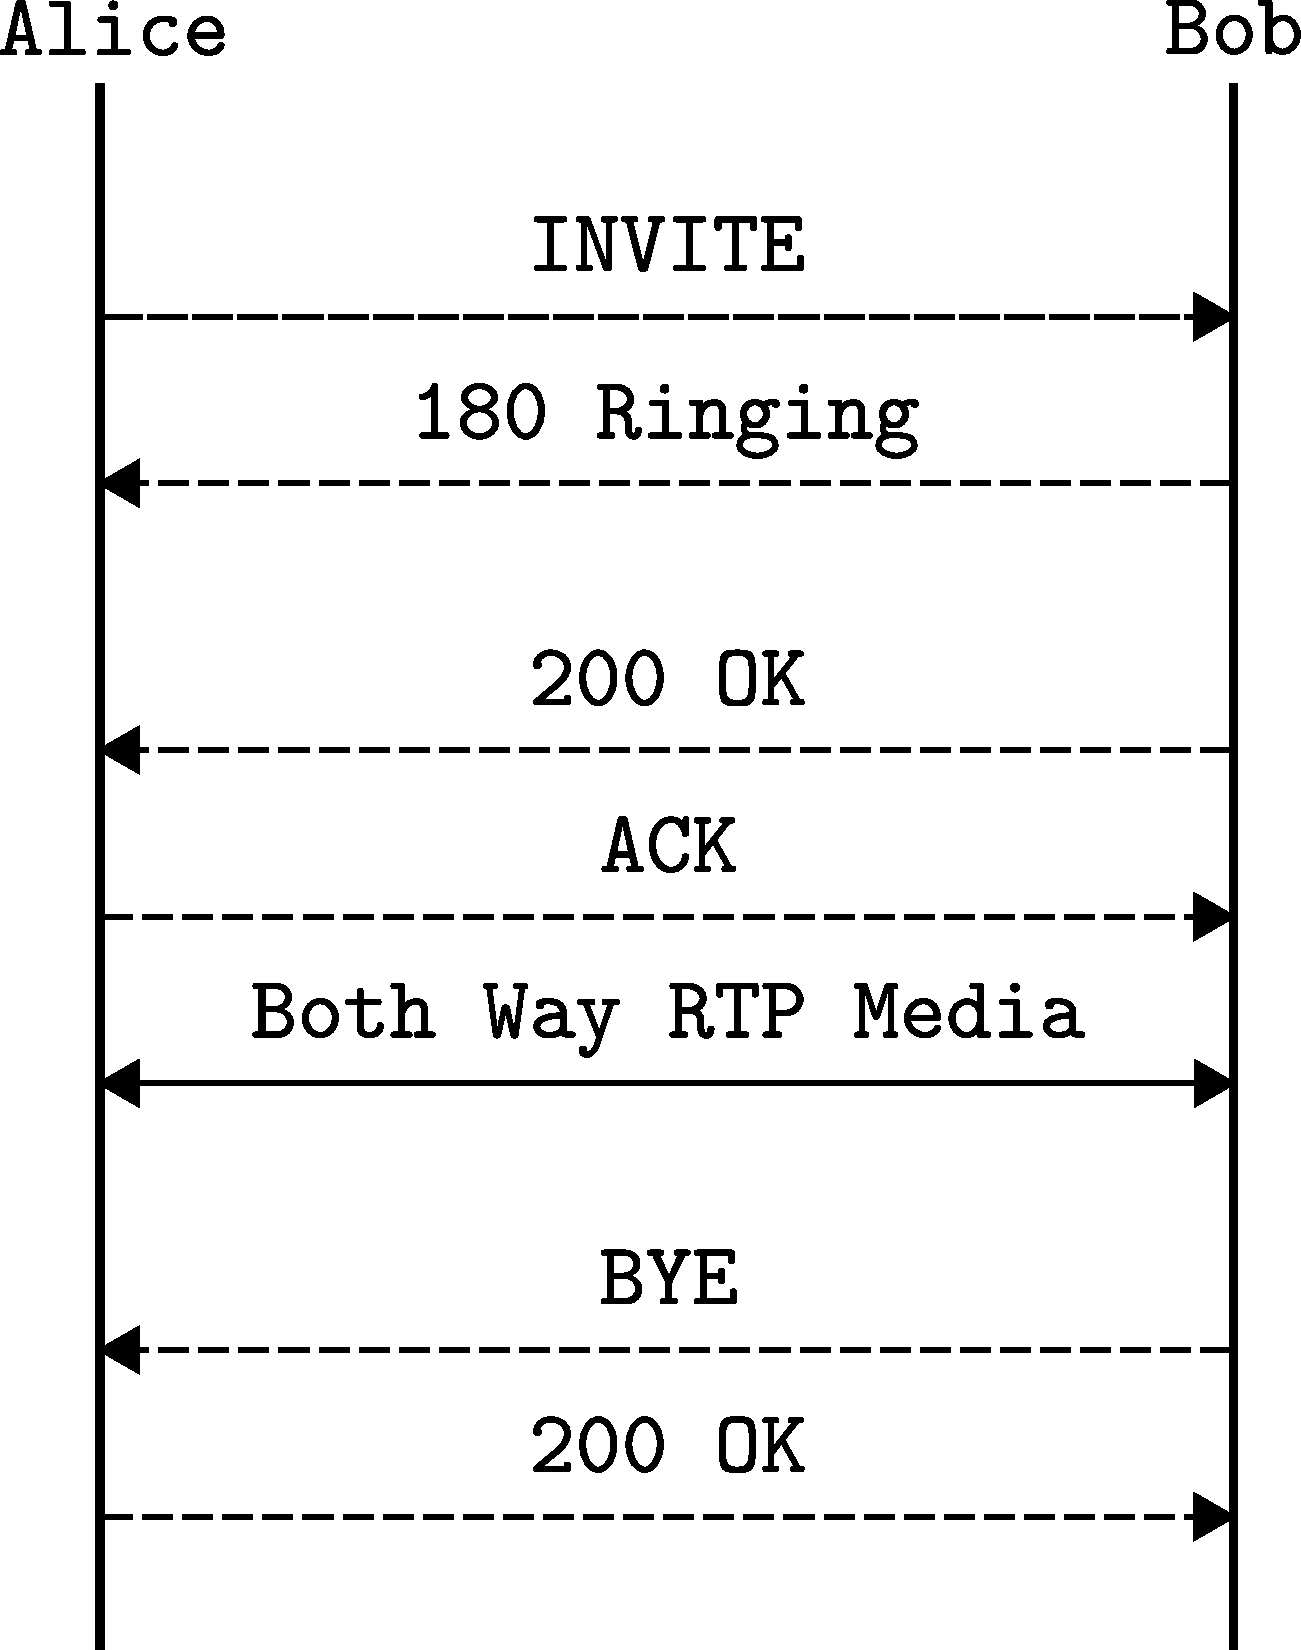
\includegraphics[width=\textwidth]{received}
    \caption{Uskutečněný hovor}
    \label{fig:received}
  \end{subfigure}%
  ~ %add desired spacing between images, e. g. ~, \quad, \qquad etc. 
  %(or a blank line to force the subfigure onto a new line)
  \begin{subfigure}[t]{0.3\textwidth}
    \centering
    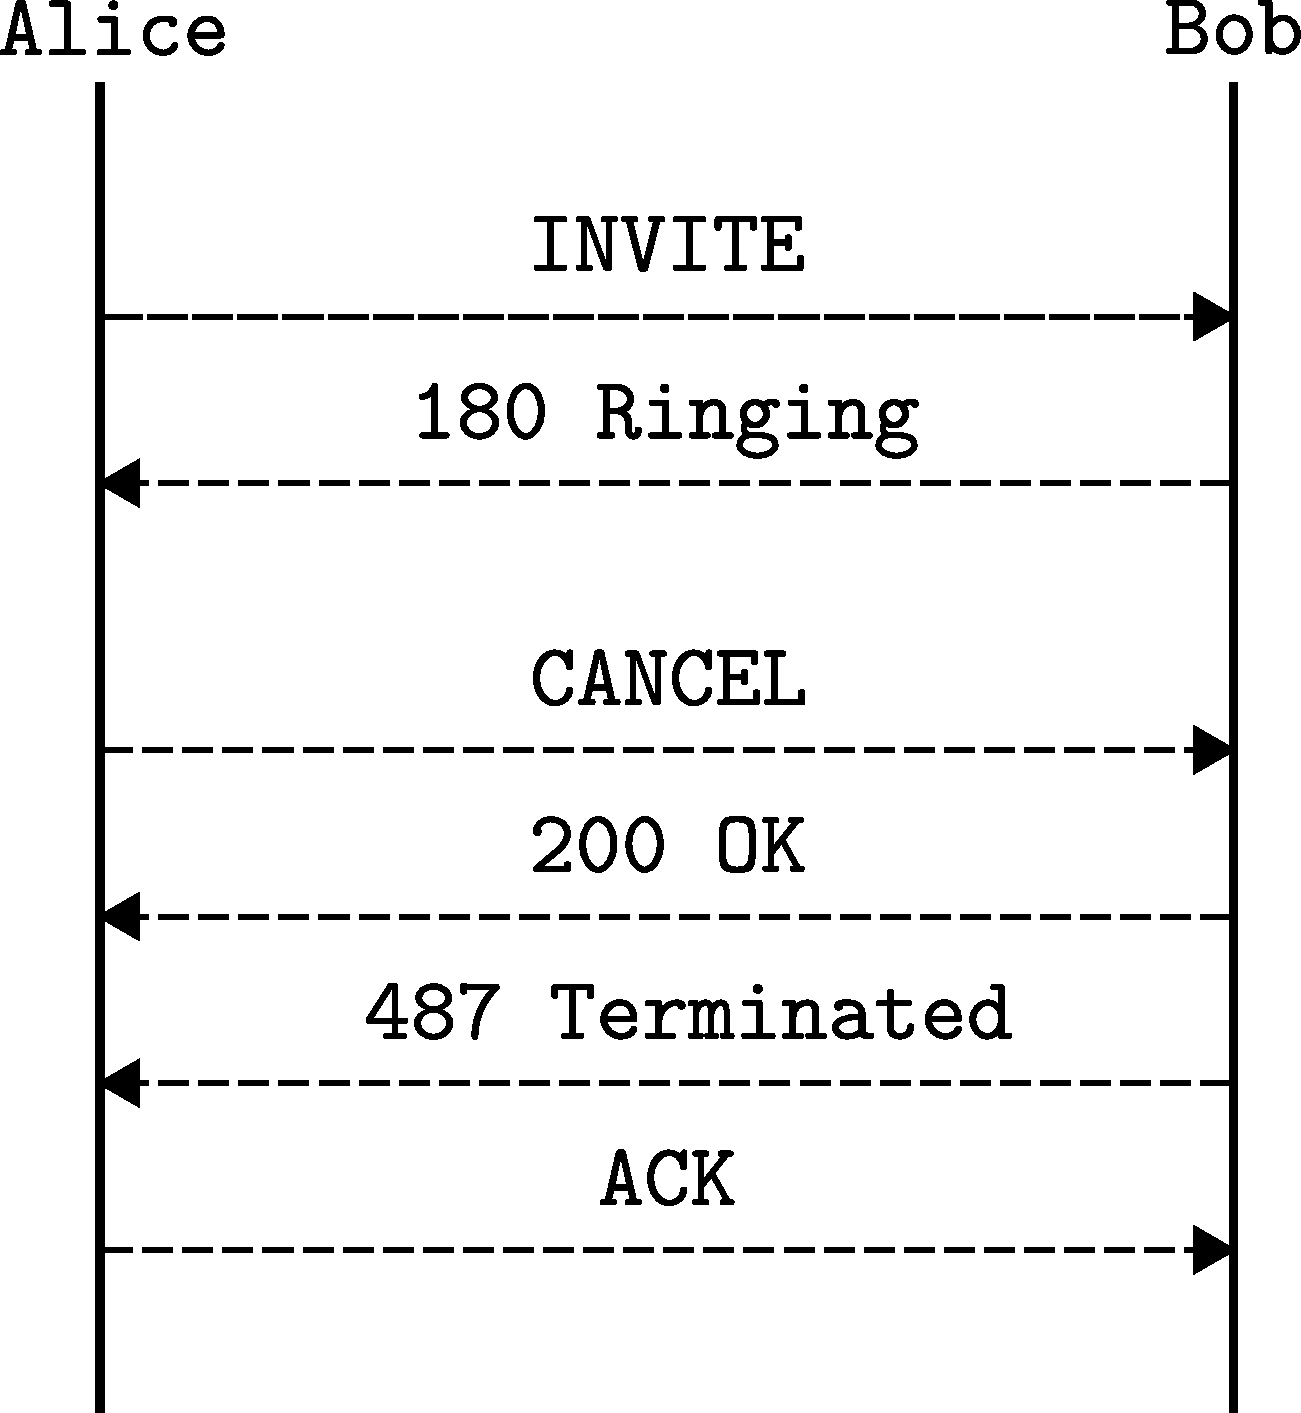
\includegraphics[width=\textwidth]{canceled}
    \caption{Zrušený hovor}
    \label{fig:canceled}
  \end{subfigure}
    ~ %add desired spacing between images, e. g. ~, \quad, \qquad etc. 
    %(or a blank line to force the subfigure onto a new line)
  \begin{subfigure}[t]{0.3\textwidth}
    \centering
    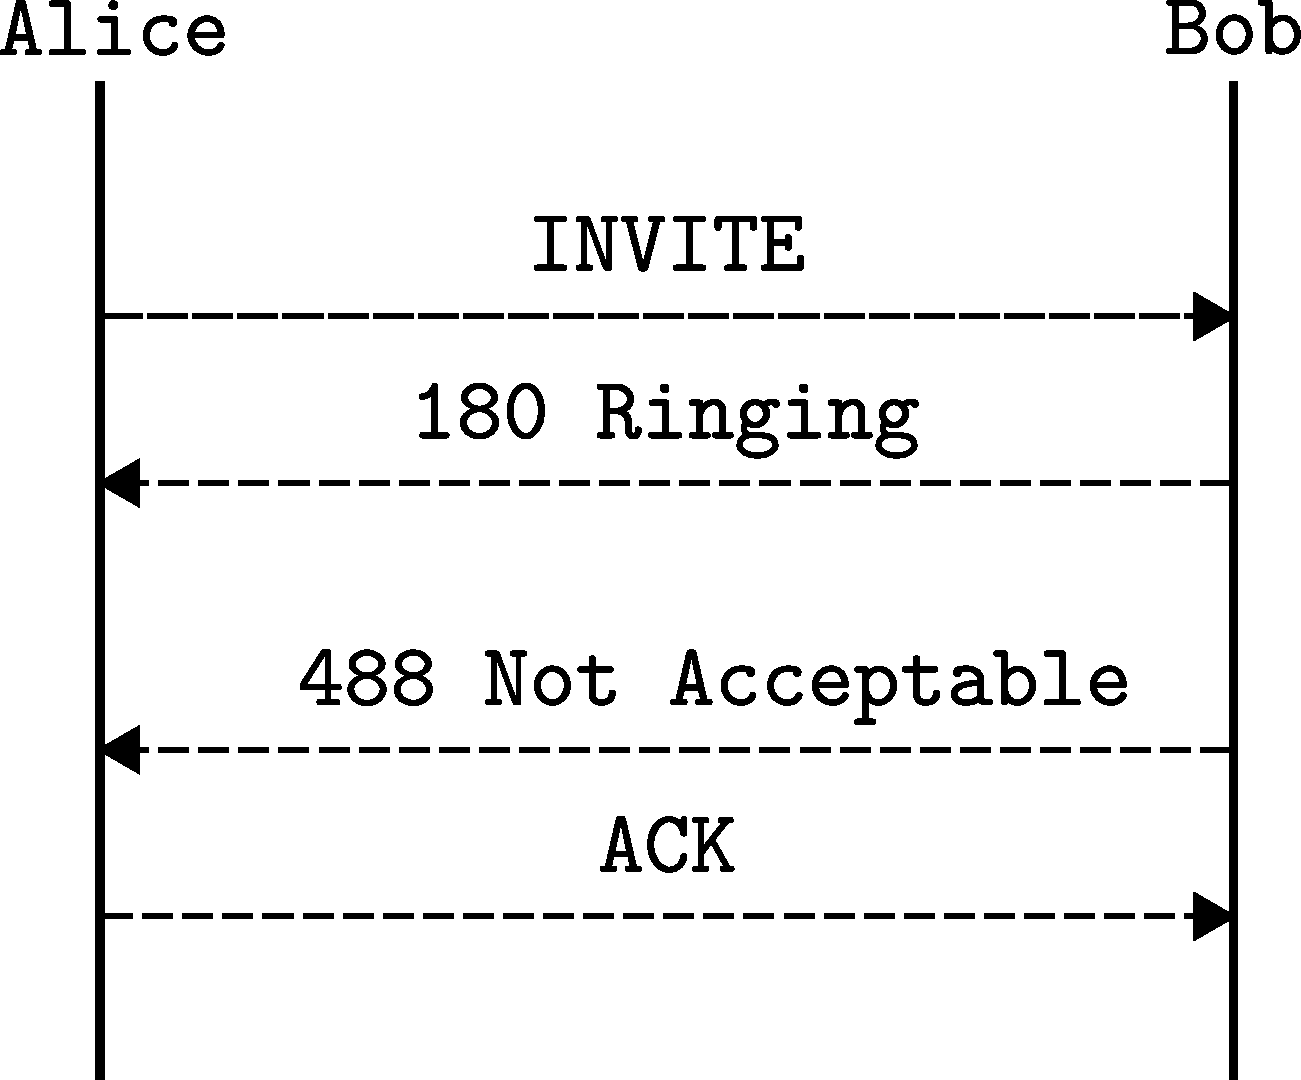
\includegraphics[width=\textwidth]{refused}
    \caption{Odmítnutý hovor}
    \label{fig:refused}
  \end{subfigure}
  \caption{Příklady komunikace \cite{rfc3665}}\label{fig:example}
\end{figure}

\section{Návrh aplikace}
Návrh aplikace je rozdělen do několika částí.
\subsection{Odchýtávaní paketů}
Naslouchání na zadaném rozhraní, použití knihovna \emph{pcap} k zachycení paketů.
\subsection{Zpracování paketů}
Z odchycených paketů je potom nutné zjistit začátek dat SIP protokolu. 
Musíme tedy určit verzi IP protokolu, abychom věděli, kde začínájí 
data transportního protokolu \cite{rfc791,rfc2460}.
Následně musíme určit transportní protokolu. V závislosti na tom, jesli se jedná
o UDP protokol nebo TCP protokol \cite{rfc768,rfc793}, určíme začátek
dat SIP protokolu.
\subsection{Rozpoznaní SIP protokolu}
Zprávu SIP protokolu rozpoznáme pomocí regulárních výrazů. Pokud
zpráva nevyhovuje formátu zprávy SIP protokolu, tak je ignorovaná. Ignorovány
jsou i zprávy SIP protokolu, které nejsou důležité pro navázaní spojení.

\subsection{Zpracování zpráv SIP protokolu}
Rozpoznané zprávy SIP protokolu je poté nutno zpracovat. Zjistí se, které
zprávy spolu souvisejí, ke~kterému požadavku SIP protokolu patří přijatá
odpověď nebo zpráva \texttt{BYE}. Při zahájení a ukončení hovoru se vytisknou informace
o hovoru, od koho je hovor, komu je určen, čas zahájení hovoru, v~případě ukončení hovoru
doplněné o délku hovoru.

\section{Implementace}
Aplikace začíná zavoláním funkce pro zpracování
parametrů aplikace. Jednotlivé parametry jsou uloženy ve struktuře \texttt{Arguments},
hodnoty parametrů \texttt{-t}, \texttt{-f}, \texttt{-u} jsou uloženy v asociativním poli, díky tomu můžeme
snadno zjistit jestli se daná položka v daném poli nachází.
Po načtení parametrů se inicializují regulární výrazy, které se využívají při~zpracování
přijatých zpráv, nastaví obsluha signálu a knihovna \emph{pcap} pro odchytávání
paketů na zadaném rozhraní. Po nastavení knihovny se zavolá funkce \texttt{pcap\_loop},
která po zachycení paketu volá obslužnou funkci, která daný paket zpracuje.

Zpracování paketů probíhá ve funkci \texttt{parsePacket}, která rozpozná verzi
IP protokolu a následně rozpozná protokol transportní vrstvy. Na základě velikosti
hlaviček jednotlivých protokolů poté určí, kde začínají vlastní data.

Pomocí regulárních výrazů se poté určí typ zprávy. U každé zprávy se z její hlavičky
zjistí její identifikátor \texttt{Call-ID}. Identifikátor je poté použit jako klíč 
k asociativnímu poli, které obsahuje seznam probíhajících hovorů.

Záznamy v tomto poli vznikají při přijetí zprávy \texttt{INVITE}. Pokud již 
záznam z daným identifikátor existuje, tak se nepřidává. Nepřidává se také, pokud
je zadán přepínač \texttt{-f}, \texttt{-t} nebo \texttt{-u}, a daný uživatel není nalezen v poli, které obsahuje
seznam uživatelů, kteří se vypisují.

Záznamy jsou mazány při přijetí zprávy \texttt{BYE}, nebo odpovědi s chybovým stavovým kódem.
Při~zachycení odpovědi je odpovídající záznam modifikován. Odpovědi, ke kterým neexistuje záznam v poli s probíhajícími hovory, jsou
ignorovány, jedná se například o odpovědi na zprávu \texttt{REGISTER}. Pokud je stavový kód 200,
vytiskne se zpráva o zahájení hovoru. V~případě chybové odpovědi se vytiskne zpráva o neuskutečněném hovoru.
Při přijetí zprávy \texttt{BYE} se vytiskne zpráva o ukončení hovoru.

\subsection{Formát výstupu}
Výstupní zprávy mají jednotný formát, který umožňuje případné zpracování pomocí skriptů.
Na prvním řádku je status, který určuje typ hovoru. Jednotlivé typy jsou \emph{Received call},
\emph{Finished call} a \emph{Refused call}, které označují začátek hovoru, konec hovoru a neuskutečněný
hovor. Na dalších řádcích jsou účastníci hovoru a čas začátku hovoru. Výpis konce hovoru navíc
obsahuje dobu trvání hovoru. V~případě neuskutečněného hovoru následuje za statusem důvod nerealizace hovoru.
Jednotlivé zprávy jsou odděleny prázdným řádkem.

\subsubsection*{Příklady výpisu:}
\begin{itemize}
  \item Začátek hovoru
  \begin{list}{\quad}{}\tt
    \item Status: Received call
    \item From: "Alice"~\textless sip:alice@atlanta.example.com\textgreater
    \item To: "Bob"~\textless sip:bob@biloxi.example.com\textgreater
    \item Time: 2012-10-29 18:51:48
  \end{list}
  \item Konec hovoru
  \begin{list}{\quad}{}\tt
    \item Status: Finished call
    \item From: "Alice"~\textless sip:alice@atlanta.example.com\textgreater
    \item To: "Bob"~\textless sip:bob@biloxi.example.com\textgreater
    \item Time: 2012-10-29 18:51:48
    \item Duration: 00:05:34
  \end{list}
  \item Neuskutečněný hovor
  \begin{list}{\quad}{}\tt
    \item Status: Refused call
    \item ~~~~~~~~487 Request Cancelled
    \item From: "Alice"~\textless sip:alice@atlanta.example.com\textgreater
    \item To: "Bob"~\textless sip:bob@biloxi.example.com\textgreater
    \item Time: 2012-10-29 17:32:16
  \end{list}
\end{itemize}

\section{Použití}
\subsection*{Synopse}
\texttt{./sip\_monitor -i \textless interface\textgreater [-a|-c] [-f \textless id\textgreater] [-t \textless id\textgreater] [-u \textless id\textgreater]}
\subsection*{Parametry}
\begin{description}
  \item[\tt -i \textless interface\textgreater] Nastaví \emph{rozhraní}, na kterém se zachycují pakety
  \item[\tt -a] Zapne výpis neuskutečněných hovorů, nelze kombinovat s parametrem \texttt{-c}
  \item[\tt -c] Vypne výpis informací o zahájení hovoru, nelze kombinovat s parametrem \texttt{-a}
  \item[\tt -f \textless id\textgreater] Vypisuje zprávy, které jsou od zadaného uživatele
  \item[\tt -t \textless id\textgreater] Vypisuje zprávy, které jsou pro zadaného uživatele
  \item[\tt -u \textless id\textgreater] Vypisuje zprávy, které jsou od nebo pro zadaného uživatele
  \item[\tt \textless id\textgreater] Jako identifikátor slouží SIP-URI, bez části "sip:"
\end{description}
\subsection*{Příklady použití:}
\begin{itemize}
  \item ./sip\_monitor -i em0
  \begin{list}{\quad}{}
    \item Zachytává pakety na rozhraní em0, na výstup vypisuje informace o zahájení a ukončení hovoru
  \end{list}
  \item ./sip\_monitor -i em0 -c -t bob@biloxi.example.com
  \begin{list}{\quad}{}
    \item Na výstup vypisuje pouze informace o ukončení hovoru, a to pouze hovorů, které jsou určeny uživateli bob@biloxi.example.com
  \end{list}
  \item ./sip\_monitor -i em0 -a -f alice@atlanta.example.com -u bob@biloxi.example.com
  \begin{list}{\quad}{}
    \item Vypisuje všechny informace, zahájení hovoru, ukončení hovoru, neuskutečněný hovor. Vypisují se pouze hovory, které jsou od uživatele alice@atlanta.example.com nebo kde je účastníkem hovoru bob@biloxi.example.com.
  \end{list}
\end{itemize}

\section{Závěr}
Testování proběhlo na referenčním virtuálním stroji. Výpis byl kontrolován
pomocí výpisu volání z programu wireshark. Při testování nebyly zjištěny 
nedostatky. Aplikace by měla splnit požadavky specifikované zadáním.

\newpage
\bibliographystyle{czplain}
\renewcommand{\refname}{Použité zdroje}
\bibliography{literatura,rfc}


\end{document}
